\chapter{วิธีการดำเนินการวิจัย}
\label{chapter:experiment}

\section{ความต้องการของระบบ}

หลังจากที่ได้สอบถามผู้ใช้งานและที่ปรึกษาระบบบีบราส พวกเรานั้นได้ความต้องการออกมาเป็นสองระบบ มีรายละเอียดดังนี้

\subsection{ระบบสามารถแสดงสถิติได้}

ระบบจะต้องสามารถแสดงสถิติการแข่งขันทุกครั้งที่ผ่านมาได้
โดยจะต้องสามารถดูสถิติการแข่งขันทดสอบทักษะการคิดเชิงคำนวณได้ทั้งระดับมัธยมต้นและมัธยมปลายของโรงเรียนของผู้ใช้งานได้
และจะต้องสามารถแสดงสถิติการแข่งขันโดยรวมของโรงเรียนทั้งหมดได้

\subsection{ระบบจัดการรายชื่อของผู้สมัคร}

ระบบจัดการรายชื่อของผู้สมัครแบ่งเป็น 3 ระบบย่อย ได้แก่

\begin{enumerate}
    \item ระบบจะต้องสามารถเพิ่มข้อมูลของผู้สมัครลงในฐานข้อมูลได้
    \item ระบบจะต้องสามารถลบข้อมูลของผู้สมัครออกจากฐานข้อมูลได้
    \item ระบบจะต้องสามารถแก้ไขข้อมูลของผู้สมัครได้
\end{enumerate}

\section{คำอธิบายของระบบ}

ระบบแสดงสถิติและจัดการรายชื่อของผู้สมัครแข่งขันทดสอบทักษะการคิดเชิงคำนวณแบ่งออกเป็น 2 ส่วน ได้แก่

\begin{enumerate}
    \item \textbf{ส่วนแสดงสถิติการแข่งขัน} ผู้ใช้สามารถเลือกที่การ์ดการแข่งขัน (Contest) เพื่อให้แสดงข้อมูลการแข่งขันได้โดยเบื้องต้นระบบจะแสดงเป็นข้อมูลสถิติการแข่งขันทั้งหมดและข้อมูลสถิติการแข่งขันของโรงเรียนของผู้ใช้งาน โดยผู้ใช้สามารถเลือกที่จะค้นหา (Search) สถิติการแข่งขันของแต่ละโรงเรียนหรือแต่ละบุคคลได้ เมื่อทำการค้นหา ระบบจะแสดงข้อมูลสถิติตามการค้นหานั้น
    \item \textbf{จัดการรายชื่อของผู้สมัครแข่งขัน} ในกรณีที่ผู้ใช้งานคือผู้ดูแลระบบ (Admin) หรือผู้ใช้งานเป็นผู้ประสานงาน (Coordinator) สามารถเลือกที่การ์ดนักเรียน (Student) เพื่อจัดการกับรายชื่อนักเรียนได้
\end{enumerate}

\newpage

\section{การออกแบบระบบจากความต้องการ}
\subsection{ภาพรวมของระบบ}

ในระบบแสดงสถิติและจัดการรายชื่อของผู้สมัครแข่งขันทดสอบทักษะการคิดเชิงคำนวณได้ใช้โครงสร้างการทำงานแบบไมโครเซอร์วิส (Microservices) \cite{WhatAreMicroservices} เพื่อให้สามารถแยกส่วนการนำส่งระบบ (Deployment) ได้ง่าย โดยมีโครงสร้างการออกแบบดังแสดงในรูปที่ \ref{fig:simplified-system-overview-diagram}

\begin{figure}[H]
    \centering
    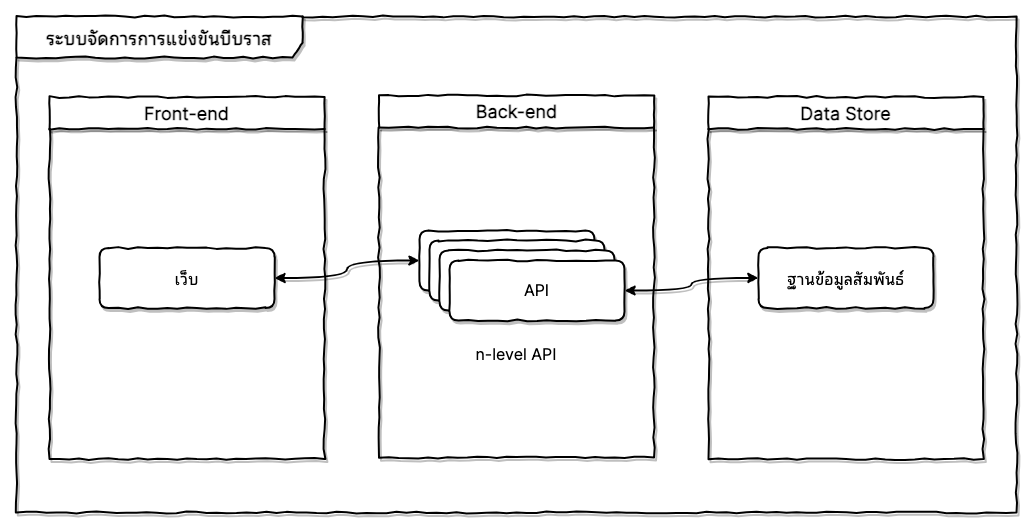
\includegraphics[width=125mm,scale=1.0]{diagrams/simplified-system-overview-diagram.png}
    \caption{ภาพรวมของระบบอย่างง่าย}
    \label{fig:simplified-system-overview-diagram}
\end{figure}

\textbf{คำอธิบาย}

สำหรับแต่ละ Use Case เว็บจะสร้างการร้องขอไปที่ API แต่ละตัว เพื่อให้สามารถทำงานได้ตามความต้องการของระบบ และสามารถอ่าน-เขียนข้อมูลลงไปที่ฐานข้อมูลสัมพันธ์ได้

\subsection{ระบบแสดงสถิติ}

ผู้จัดทำได้สกัดความต้องการของระบบแสดงสถิติออกมาเป็น Use Case ทั้งหมด 6 อัน โดยจะแบ่งเป็น 2 บทบาทการใช้งาน คือ ผู้ประสานงานและผู้ดูแลระบบ ดังแสดงในรูปที่ \ref{fig:package-display-stats-diagram}
โดยในระบบแสดงสถิติจะประกอบไปด้วย Use Case ดังนี้
\begin{enumerate}
    \item Use case ดูข้อมูลสถิติการทดสอบ ดังแสดงในตารางที่ \ref{tab:usecase-read-stats}
    \item Use case ส่งออกข้อมูลสถิติการทดสอบ ดังแสดงในตารางที่ \ref{tab:usecase-export-stats}
    \item Use case แก้ไขข้อมูลสถิติการทดสอบ ดังแสดงในตารางที่ \ref{tab:usecase-edit-stats}
    \item Use case ส่งออกชื่อผู้ใช้และรหัสผ่านสำหรับ Moodle ดังแสดงในตารางที่ \ref{tab:usecase-export-moodle-student}
    \item Use case ดูคะแนนการทดสอบ ดังแสดงในตารางที่ \ref{tab:usecase-read-result}
    \item Use case เพิ่มข้อมูลสถิติการทดสอบ ดังแสดงในตารางที่ \ref{tab:usecase-import-stats}
\end{enumerate}

\begin{figure}[H]
    \centering
    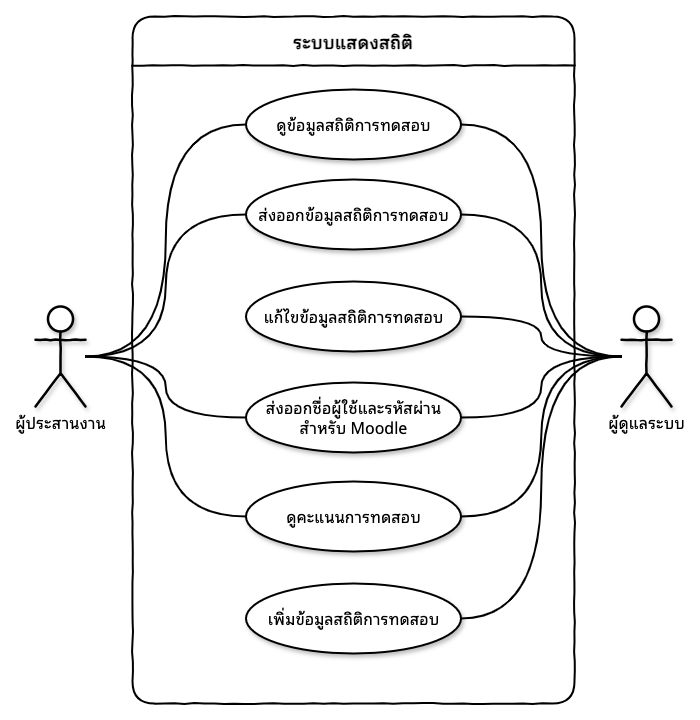
\includegraphics[width=100mm,scale=1.0]{diagrams/package-display-stats.png}
    \caption{แผนภาพแสดงระบบแสดงสถิติ}
    \label{fig:package-display-stats-diagram}
\end{figure}

\subsection{ระบบจัดการรายชื่อผู้เข้าแข่งขัน}

ผู้จัดทำได้สกัดความต้องการของระบบจัดการรายชื่อผู้เข้าแข่งขันออกมาเป็น Use Case ทั้งหมด 11 อัน โดยจะแบ่งเป็น 2 บทบาทการใช้งาน คือ ผู้ประสานงานและผู้ดูแลระบบ ดังแสดงในรูปที่ \ref{fig:package-manage-students-diagram}
โดยในระบบจัดการรายชื่อผู้เข้าแข่งขันจะประกอบไปด้วย Use Case ดังนี้
\begin{enumerate}
    \item Use case ค้นหารายชื่อนักเรียน ดังแสดงในตารางที่ \ref{tab:usecase-search-student}
    \item Use case อ่านรายชื่อนักเรียน ดังแสดงในตารางที่ \ref{tab:usecase-read-student}
    \item Use case ลบรายชื่อนักเรียน ดังแสดงในตารางที่ \ref{tab:usecase-remove-student}
    \item Use case แก้ไขข้อมูลนักเรียน ดังแสดงในตารางที่ \ref{tab:usecase-edit-student}
    \item Use case เพิ่มรายชื่อนักเรียน ดังแสดงในตารางที่ \ref{tab:usecase-create-student}
    \item Use case สร้างชื่อผู้ใช้และรหัสผ่านสำหรับ Moodle ดังแสดงในตารางที่ \ref{tab:usecase-generate-user}
    \item Use case เพิ่มรายชื่อนักเรียนแบบกลุ่ม ดังแสดงในตารางที่ \ref{tab:usecase-create-batch-student}
    \item Use case อ่านข้อมูลประเภทการทดสอบ ดังแสดงในตารางที่ \ref{tab:usecase-read-contest}
    \item Use case เพิ่มประเภทการทดสอบ ดังแสดงในตารางที่ \ref{tab:usecase-create-contest}
    \item Use case ส่งออกรายชื่อนักเรียน ดังแสดงในตารางที่ \ref{tab:usecase-export-student}
    \item Use case ลบประเภทการทดสอบ ดังแสดงในตารางที่ \ref{tab:usecase-remove-contest}
\end{enumerate}

\begin{figure}[H]
    \centering
    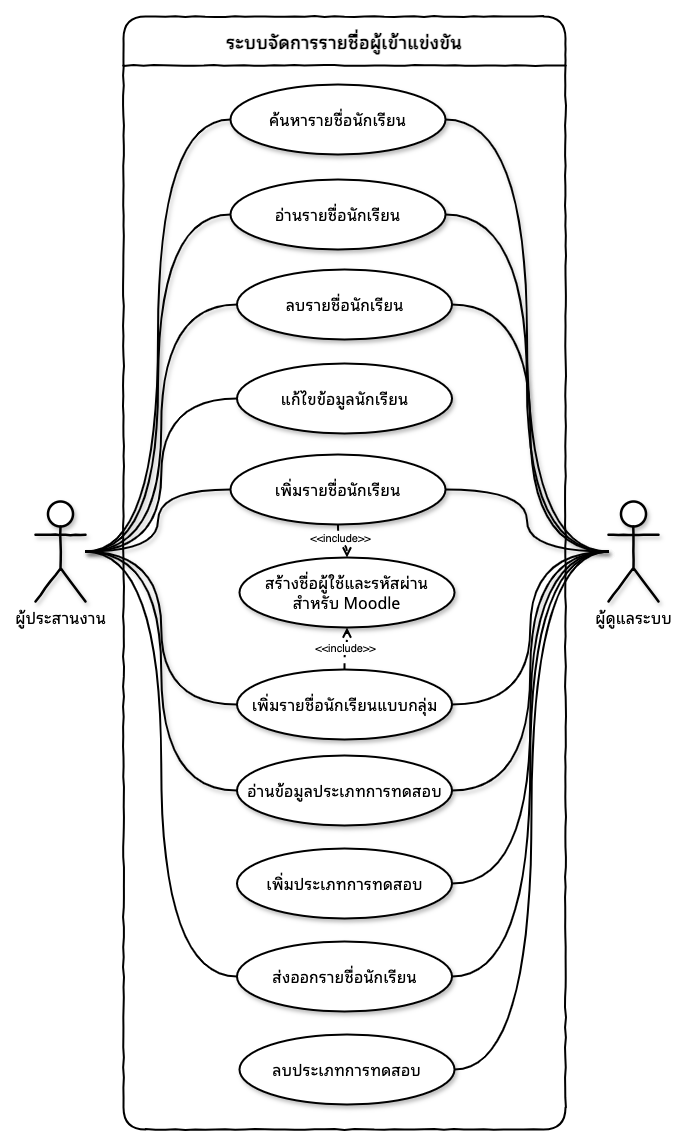
\includegraphics[width=100mm,scale=1.0]{diagrams/package-manage-students.png}
    \caption{แผนภาพแสดงระบบจัดการรายชื่อผู้เข้าแข่งขัน}
    \label{fig:package-manage-students-diagram}
\end{figure}

\subsection{Use Case Specification}

\begin{table}[H]
    \caption{Use Case อ่านสถิติการทดสอบ}
    \label{tab:usecase-read-stats}
    \begin{tabularx}{\textwidth}{ | p{3cm} | X | }
    \hline
    \textbf{Use Case} & อ่านสถิติการทดสอบ \\
    \hline
    \textbf{Actor} & ผู้ประสานงาน, ผู้ดูแลระบบ \\
    \hline
    \textbf{Description} & ผู้ใช้สามารถอ่านสถิติการทดสอบได้ \\
    \hline
    \textbf{Pre-Condition} & - \\
    \hline
    \textbf{Post-Condition} & - \\
    \hline
    \end{tabularx}
    \begin{tabularx}{\textwidth}{ | X | X | X | }
    \multicolumn{3}{|c|}{\textbf{Flow of Events}} \\
    \hline
    \multicolumn{1}{|c|}{\textbf{General}} & \multicolumn{1}{|c|}{\textbf{Actor Action}} & \multicolumn{1}{|c|}{\textbf{System Response}} \\
    \hline
    1. ผู้ใช้คลิกที่การ์ดประเภทการแข่งขันเพื่อเข้าสู่ Use Case นี้ &  &  \\
    \hline
    & 2. ผู้ใช้เลือกประเภทการแข่งขันที่ต้องการดูสถิติ & \\
    \hline
    & 3. ผู้ใช้คลิกดูสถิติ & \\
    \hline
    & & 4. ระบบสร้างการร้องขอข้อมูลสถิติแข่งขันจากฐานข้อมูลสัมพันธ์และสร้างกราฟข้อมูลให้ผู้ใช้ \\
    \hline
    \end{tabularx}
\end{table}

\begin{table}[H]
    \caption{Use Case ส่งออกข้อมูลสถิติการทดสอบ}
    \label{tab:usecase-export-stats}
    \begin{tabularx}{\textwidth}{ | p{3cm} | X | }
    \hline
    \textbf{Use Case} & ส่งออกข้อมูลสถิติการทดสอบ \\
    \hline
    \textbf{Actor} & ผู้ประสานงาน, ผู้ดูแลระบบ \\
    \hline
    \textbf{Description} & ผู้ใช้สามารถส่งออกข้อมูลสถิติการทดสอบได้ \\
    \hline
    \textbf{Pre-Condition} & - \\
    \hline
    \textbf{Post-Condition} & - \\
    \hline
    \end{tabularx}
    \begin{tabularx}{\textwidth}{ | X | X | X | }
    \multicolumn{3}{|c|}{\textbf{Flow of Events}} \\
    \hline
    \multicolumn{1}{|c|}{\textbf{General}} & \multicolumn{1}{|c|}{\textbf{Actor Action}} & \multicolumn{1}{|c|}{\textbf{System Response}} \\
    \hline
    1. ผู้ใช้คลิกที่การ์ดประเภทการแข่งขันเพื่อเข้าสู่ Use Case นี้ &  &  \\
    \hline
    & 2. ผู้ใช้เลือกประเภทการแข่งขันที่ต้องการส่งออก & \\
    \hline
    & 3. ผู้ใช้คลิกดูสถิติ & \\
    \hline
    & 4. ผู้ใช้คลิกส่งออกข้อมูลสถิติ & \\
    \hline
    & & 5. ระบบสร้างการร้องขอข้อมูลสถิติแข่งขันจากฐานข้อมูลสัมพันธ์และดาวน์โหลดให้ผู้ใช้ \\
    \hline
    \end{tabularx}
\end{table}

\begin{table}[H]
    \caption{Use Case แก้ไขข้อมูลสถิติการทดสอบ}
    \label{tab:usecase-edit-stats}
    \begin{tabularx}{\textwidth}{ | p{3cm} | X | }
    \hline
    \textbf{Use Case} & แก้ไขข้อมูลสถิติการทดสอบ \\
    \hline
    \textbf{Actor} & ผู้ดูแลระบบ \\
    \hline
    \textbf{Description} & ผู้ดูแลระบบสามารถแก้ไขข้อมูลสถิติการทดสอบได้ \\
    \hline
    \textbf{Pre-Condition} & - \\
    \hline
    \textbf{Post-Condition} & - \\
    \hline
    \end{tabularx}
    \begin{tabularx}{\textwidth}{ | X | X | X | }
    \multicolumn{3}{|c|}{\textbf{Flow of Events}} \\
    \hline
    \multicolumn{1}{|c|}{\textbf{General}} & \multicolumn{1}{|c|}{\textbf{Actor Action}} & \multicolumn{1}{|c|}{\textbf{System Response}} \\
    \hline
    1. ผู้ดูแลระบบคลิกที่การ์ดประเภทการแข่งขันเพื่อเข้าสู่ Use Case นี้ &  &  \\
    \hline
    & 2. ผู้ดูแลระบบคลิกปุ่มเพิ่มผลลัพธ์การแข่งขันเพื่อเขียนทับสถิติเดิม &  \\
    \hline
    & 3. ผู้ดูแลเพิ่มไฟล์ผลลัพธ์การแข่งขันในรูปแบบ CSV  &  \\
    \hline
    & 4. ผู้ดูแลระบบกดปุ่มเพิ่ม &  \\
    \hline
    & & 5. ระบบแก้ไขข้อมูลสถิติการทดสอบลงในฐานข้อมูลสัมพันธ์ \\
    \hline
    & & 6. ระบบแจ้งเตือนการเพิ่มสถิติการทดสอบสำเร็จแก่ผู้ดูแลระบบ \\
    \hline
    \end{tabularx}
\end{table}

\begin{table}[H]
    \caption{Use Case ส่งออกชื่อผู้ใช้และรหัสผ่านสำหรับ Moodle}
    \label{tab:usecase-export-moodle-student}
    \begin{tabularx}{\textwidth}{ | p{3cm} | X | }
    \hline
    \textbf{Use Case} & ส่งออกชื่อผู้ใช้และรหัสผ่านสำหรับ Moodle \\
    \hline
    \textbf{Actor} & ผู้ประสานงาน, ผู้ดูแลระบบ \\
    \hline
    \textbf{Description} & ผู้ใช้สามารถส่งออกชื่อผู้ใช้และรหัสผ่านสำหรับ Moodle ได้ \\
    \hline
    \textbf{Pre-Condition} & - \\
    \hline
    \textbf{Post-Condition} & - \\
    \hline
    \end{tabularx}
    \begin{tabularx}{\textwidth}{ | X | X | X | }
    \multicolumn{3}{|c|}{\textbf{Flow of Events}} \\
    \hline
    \multicolumn{1}{|c|}{\textbf{General}} & \multicolumn{1}{|c|}{\textbf{Actor Action}} & \multicolumn{1}{|c|}{\textbf{System Response}} \\
    \hline
    1. ผู้ดูแลระบบคลิกที่การ์ดประเภทการแข่งขันเพื่อเข้าสู่ Use Case นี้ &  &  \\
    \hline
    & 2. ผู้ใช้เลือกประเภทการแข่งขันที่ต้องส่งออก  &  \\
    \hline
    & 3. ผู้ใช้คลิกเลือกรูปแบบไฟล์ที่ต้องการ  &  \\
    \hline
    & & 4. ระบบเลือกชื่อผู้ใช้และรหัสผ่านของนักเรียนของโรงเรียนผู้ประสานงานจากฐานข้อมูลสัมพันธ์ \\
    \hline
    & & 5. ระบบแปลงไฟล์เป็นรูปแบบเดียวกับที่ผู้ใช้เลือก \\
    \hline
    & & 6. ระบบดาวน์โหลดให้ผู้ใช้ \\
    \hline
    \end{tabularx}
\end{table}

\begin{table}[H]
    \caption{Use Case ดูคะแนนการทดสอบ}
    \label{tab:usecase-read-result}
    \begin{tabularx}{\textwidth}{ | p{3cm} | X | }
    \hline
    \textbf{Use Case} & ดูคะแนนการทดสอบ \\
    \hline
    \textbf{Actor} & ผู้ประสานงาน, ผู้ดูแลระบบ \\
    \hline
    \textbf{Description} & ผู้ใช้สามารถดูคะแนนการทดสอบได้ \\
    \hline
    \textbf{Pre-Condition} & - \\
    \hline
    \textbf{Post-Condition} & - \\
    \hline
    \end{tabularx}
    \begin{tabularx}{\textwidth}{ | X | X | X | }
    \multicolumn{3}{|c|}{\textbf{Flow of Events}} \\
    \hline
    \multicolumn{1}{|c|}{\textbf{General}} & \multicolumn{1}{|c|}{\textbf{Actor Action}} & \multicolumn{1}{|c|}{\textbf{System Response}} \\
    \hline
    1. ผู้ใช้คลิกที่การ์ดประเภทการแข่งขันเพื่อเข้าสู่ Use Case นี้ &  &  \\
    \hline
    & 2. ผู้ใช้เลือกประเภทการแข่งขันที่ต้องการดูคะแนนการทดสอบ & \\
    \hline
    & & 4. ระบบสร้างการร้องขอข้อมูลคะแนนจากฐานข้อมูลสัมพันธ์และสร้างตารางข้อมูลให้ผู้ใช้ \\
    \hline
    \end{tabularx}
\end{table}

\begin{table}[H]
    \caption{Use Case เพิ่มข้อมูลสถิติการทดสอบ}
    \label{tab:usecase-import-stats}
    \begin{tabularx}{\textwidth}{ | p{3cm} | X | }
    \hline
    \textbf{Use Case} & เพิ่มข้อมูลสถิติการทดสอบ \\
    \hline
    \textbf{Actor} & ผู้ดูแลระบบ \\
    \hline
    \textbf{Description} & ผู้ดูแลระบบสามารถเพิ่มข้อมูลสถิติการทดสอบได้ \\
    \hline
    \textbf{Pre-Condition} & - \\
    \hline
    \textbf{Post-Condition} & - \\
    \hline
    \end{tabularx}
    \begin{tabularx}{\textwidth}{ | X | X | X | }
    \multicolumn{3}{|c|}{\textbf{Flow of Events}} \\
    \hline
    \multicolumn{1}{|c|}{\textbf{General}} & \multicolumn{1}{|c|}{\textbf{Actor Action}} & \multicolumn{1}{|c|}{\textbf{System Response}} \\
    \hline
    1. ผู้ดูแลระบบคลิกที่การ์ดประเภทการแข่งขันเพื่อเข้าสู่ Use Case นี้ &  &  \\
    \hline
    & 2. ผู้ดูแลระบบคลิกปุ่มเพิ่มผลลัพธ์การแข่งขัน  &  \\
    \hline
    & 3. ผู้ดูแลเพิ่มไฟล์ผลลัพธ์การแข่งขันในรูปแบบ CSV  &  \\
    \hline
    & 4. ผู้ดูแลระบบกดปุ่มเพิ่ม &  \\
    \hline
    & & 5. ระบบเพิ่มข้อมูลสถิติการทดสอบลงในฐานข้อมูลสัมพันธ์ \\
    \hline
    & & 6. ระบบแจ้งเตือนการเพิ่มสถิติการทดสอบสำเร็จแก่ผู้ดูแลระบบ \\
    \hline
    \end{tabularx}
\end{table}

\begin{table}[H]
    \caption{Use Case ค้นหารายชื่อนักเรียน}
    \label{tab:use-case-search-student}
    \begin{tabularx}{\textwidth}{ | p{3cm} | X | }
    \hline
    \textbf{Use Case} & ค้นหารายชื่อนักเรียน \\
    \hline
    \textbf{Actor} & ผู้ประสานงาน, ผู้ดูแลระบบ \\
    \hline
    \textbf{Description} & ผู้ใช้สามารถค้นหารายชื่อนักเรียนได้ \\
    \hline
    \textbf{Pre-Condition} & - \\
    \hline
    \textbf{Post-Condition} & - \\
    \hline
    \end{tabularx}
    \begin{tabularx}{\textwidth}{ | X | X | X | }
    \multicolumn{3}{|c|}{\textbf{Flow of Events}} \\
    \hline
    \multicolumn{1}{|c|}{\textbf{General}} & \multicolumn{1}{|c|}{\textbf{Actor Action}} & \multicolumn{1}{|c|}{\textbf{System Response}} \\
    \hline
    1. ผู้ใช้คลิกที่การ์ดนักเรียนเพื่อเข้าสู่ Use Case นี้ &  &  \\
    \hline
    & 2. ผู้ใช้กรอกข้อมูลที่ต้องการค้นหา & \\
    \hline
    & 3. ผู้ใช้กดปุ่มค้นหา &  \\
    \hline
    & & 4. ระบบแสดงรายชื่อนักเรียนที่ตรงกับเงื่อนไขการค้นหา \\
    \hline
    \end{tabularx}
\end{table}

\begin{table}[H]
    \caption{Use Case อ่านรายชื่อนักเรียน}
    \label{tab:use-case-read-student}
    \begin{tabularx}{\textwidth}{ | p{3cm} | X | }
    \hline
    \textbf{Use Case} & อ่านรายชื่อนักเรียน \\
    \hline
    \textbf{Actor} & ผู้ประสานงาน, ผู้ดูแลระบบ \\
    \hline
    \textbf{Description} & ผู้ใช้สามารถอ่านรายชื่อนักเรียนได้ \\
    \hline
    \textbf{Pre-Condition} & - \\
    \hline
    \textbf{Post-Condition} & - \\
    \hline
    \end{tabularx}
    \begin{tabularx}{\textwidth}{ | X | X | X | }
    \multicolumn{3}{|c|}{\textbf{Flow of Events}} \\
    \hline
    \multicolumn{1}{|c|}{\textbf{General}} & \multicolumn{1}{|c|}{\textbf{Actor Action}} & \multicolumn{1}{|c|}{\textbf{System Response}} \\
    \hline
    1. ผู้ใช้คลิกที่การ์ดนักเรียนเพื่อเข้าสู่ Use Case นี้ &  &  \\
    \hline
    & & 2. ระบบสร้างการร้องขอข้อมูลรายชื่อนักเรียนจากฐานข้อมูลสัมพันธ์และสร้างเป็นตารางรายชื่อให้ผู้ใช้ \\
    \hline
    \end{tabularx}
\end{table}

\begin{table}[H]
    \caption{Use Case ลบรายชื่อนักเรียน}
    \label{tab:use-case-remove-student}
    \begin{tabularx}{\textwidth}{ | p{3cm} | X | }
    \hline
    \textbf{Use Case} & ลบรายชื่อนักเรียน \\
    \hline
    \textbf{Actor} & ผู้ประสานงาน, ผู้ดูแลระบบ \\
    \hline
    \textbf{Description} & ผู้ใช้สามารถลบรายชื่อนักเรียนได้ \\
    \hline
    \textbf{Pre-Condition} & - \\
    \hline
    \textbf{Post-Condition} & - \\
    \hline
    \end{tabularx}
    \begin{tabularx}{\textwidth}{ | X | X | X | }
    \multicolumn{3}{|c|}{\textbf{Flow of Events}} \\
    \hline
    \multicolumn{1}{|c|}{\textbf{General}} & \multicolumn{1}{|c|}{\textbf{Actor Action}} & \multicolumn{1}{|c|}{\textbf{System Response}} \\
    \hline
    1. ผู้ใช้คลิกที่การ์ดนักเรียนเพื่อเข้าสู่ Use Case นี้ & & \\
    \hline
    & 2. ผู้ใช้คลิกที่ปุ่มถังขยะในแถวของนักเรียนที่ต้องการลบ & \\
    \hline
    & 3. ผู้ใช้คลิกที่ปุ่มยืนยัน & \\
    \hline
    & & 4. ระบบทำการลบนักเรียนจากฐานข้อมูลสัมพันธ์ \\
    \hline
    & & 5. ระบบแจ้งเตือนการลบนักเรียนสำเร็จให้แก่ผู้ใช้ \\
    \hline
    \end{tabularx}
\end{table}

\begin{table}[H]
    \caption{Use Case แก้ไขข้อมูลนักเรียน}
    \label{tab:usecase-edit-student}
    \begin{tabularx}{\textwidth}{ | p{3cm} | X | }
    \hline
    \textbf{Use Case} & แก้ไขข้อมูลนักเรียน \\
    \hline
    \textbf{Actor} & ผู้ประสานงาน \\
    \hline
    \textbf{Description} & ผู้ใช้สามารถแก้ไขข้อมูลนักเรียนได้ \\
    \hline
    \textbf{Pre-Condition} & - \\
    \hline
    \textbf{Post-Condition} & - \\
    \hline
    \end{tabularx}
    \begin{tabularx}{\textwidth}{ | X | X | X | }
    \multicolumn{3}{|c|}{\textbf{Flow of Events}} \\
    \hline
    \multicolumn{1}{|c|}{\textbf{General}} & \multicolumn{1}{|c|}{\textbf{Actor Action}} & \multicolumn{1}{|c|}{\textbf{System Response}} \\
    \hline
    1. ผู้ใช้คลิกที่การ์ดนักเรียนเพื่อเข้าสู่ Use Case นี้ & & \\
    \hline
    & 2. ผู้ใช้คลิกที่ปุ่มแก้ไขของนักเรียนที่ต้องการ & \\
    \hline
    & 3. ผู้ใช้กรอกข้อมูลของที่ต้องการแก้ไขลงในกล่องข้อความแต่ละกล่อง & \\
    \hline
    & 4. ผู้ใช้คลิกที่ปุ่มแก้ไข & \\
    \hline
    & & 5. ระบบแก้ไขข้อมูลนักเรียนลงในฐานข้อมูลสัมพันธ์ \\
    \hline
    & & 6. ระบบแจ้งเตือนการแก้ไขข้อมูลนักเรียนสำเร็จให้แก่ผู้ใช้ \\
    \hline
    \end{tabularx}
\end{table}

\begin{table}[H]
    \caption{Use Case เพิ่มรายชื่อนักเรียน}
    \label{tab:use-case-create-student}
    \begin{tabularx}{\textwidth}{ | p{3cm} | X | }
    \hline
    \textbf{Use Case} & เพิ่มรายชื่อนักเรียน \\
    \hline
    \textbf{Actor} & ผู้ประสานงาน, ผู้ดูแลระบบ \\
    \hline
    \textbf{Description} & ผู้ใช้สามารถเพิ่มรายชื่อนักเรียนได้ \\
    \hline
    \textbf{Pre-Condition} & - \\
    \hline
    \textbf{Post-Condition} & - \\
    \hline
    \end{tabularx}
    \begin{tabularx}{\textwidth}{ | X | X | X | }
    \multicolumn{3}{|c|}{\textbf{Flow of Events}} \\
    \hline
    \multicolumn{1}{|c|}{\textbf{General}} & \multicolumn{1}{|c|}{\textbf{Actor Action}} & \multicolumn{1}{|c|}{\textbf{System Response}} \\
    \hline
    1. ผู้ใช้คลิกที่การ์ดนักเรียนเพื่อเข้าสู่ Use Case นี้ & & \\
    \hline
    & 2. ผู้ใช้คลิกที่ปุ่มเพิ่มนักเรียน & \\
    \hline
    & 3. ผู้ใช้กรอกข้อมูลของนักเรียนในกล่องข้อความแต่ละกล่อง & \\
    \hline
    & 4. ผู้ใช้คลิกที่ปุ่มเพิ่ม & \\
    \hline
    & & 5. ระบบเพิ่มนักเรียนลงในฐานข้อมูลสัมพันธ์ \\
    \hline
    & & 6. ระบบแจ้งเตือนการเพิ่มนักเรียนสำเร็จให้แก่ผู้ใช้ \\
    \hline
    \end{tabularx}
\end{table}

\begin{table}[H]
    \caption{Use Case สร้างชื่อผู้ใช้และรหัสผ่านสำหรับ Moodle}
    \label{tab:usecase-generate-user}
    \begin{tabularx}{\textwidth}{ | p{3cm} | X | }
    \hline
    \textbf{Use Case} & สร้างชื่อผู้ใช้และรหัสผ่านสำหรับ Moodle \\
    \hline
    \textbf{Actor} & - \\
    \hline
    \textbf{Description} & ระบบสามารถสร้างชื่อผู้ใช้และรหัสผ่านสำหรับ Moodle ได้ \\
    \hline
    \textbf{Pre-Condition} & - \\
    \hline
    \textbf{Post-Condition} & - \\
    \hline
    \end{tabularx}
    \begin{tabularx}{\textwidth}{ | X | X | X | }
    \multicolumn{3}{|c|}{\textbf{Flow of Events}} \\
    \hline
    \multicolumn{1}{|c|}{\textbf{General}} & \multicolumn{1}{|c|}{\textbf{Actor Action}} & \multicolumn{1}{|c|}{\textbf{System Response}} \\
    \hline
    1. Use Case นี้จะเริ่มเมื่อถูกเรียกใช้จากการสร้างนักเรียนใหม่ในระบบ & & \\
    \hline
    & & 2. ระบบทำการจองชื่อผู้ใช้และสร้างรหัสผ่านใหม่ให้กับนักเรียน \\
    \hline
    & & 3. ระบบบันทึกชื่อผู้ใช้และรหัสผ่านลงในฐานข้อมูลสัมพันธ์ \\
    \hline
    \end{tabularx}
\end{table}

\begin{table}[H]
    \caption{Use Case เพิ่มรายชื่อนักเรียนแบบกลุ่ม}
    \label{tab:use-case-create-batch-student}
    \begin{tabularx}{\textwidth}{ | p{3cm} | X | }
    \hline
    \textbf{Use Case} & เพิ่มรายชื่อนักเรียนแบบกลุ่ม \\
    \hline
    \textbf{Actor} & ผู้ประสานงาน, ผู้ดูแลระบบ \\
    \hline
    \textbf{Description} & ผู้ใช้สามารถเพิ่มรายชื่อนักเรียนแบบกลุ่มได้ \\
    \hline
    \textbf{Pre-Condition} & ผู้ใช้ต้องทำการเพิ่มข้อมูลนักเรียนลงไปในไฟล์ Excel ในเทมเพลตที่จัดเตรียมไว้ให้ \\
    \hline
    \textbf{Post-Condition} & - \\
    \hline
    \end{tabularx}
    \begin{tabularx}{\textwidth}{ | X | X | X | }
    \multicolumn{3}{|c|}{\textbf{Flow of Events}} \\
    \hline
    \multicolumn{1}{|c|}{\textbf{General}} & \multicolumn{1}{|c|}{\textbf{Actor Action}} & \multicolumn{1}{|c|}{\textbf{System Response}} \\
    \hline
    1. ผู้ใช้คลิกที่การ์ดนักเรียนเพื่อเข้าสู่ Use Case นี้ & & \\
    \hline
    & 2. ผู้ใช้คลิกที่ปุ่มนำเข้านักเรียน & \\
    \hline
    & 3. ผู้ใช้คลิกที่ปุ่มอัพโหลดไฟล์ และเลือกไฟล์ Excel ที่ได้จัดเตรียมไว้ & \\
    \hline
    & 4. ผู้ใช้เลือกภาษาการสอบของนักเรียนที่ต้องการเพิ่ม & \\
    \hline
    & 5. ผู้ใช้คลิกที่ปุ่มนำเข้า & \\
    \hline
    & & 6. ระบบเพิ่มนักเรียนลงในฐานข้อมูลสัมพันธ์ \\
    \hline
    & & 7. ระบบแจ้งเตือนการเพิ่มนักเรียนสำเร็จให้แก่ผู้ใช้ \\
    \hline
    \end{tabularx}
\end{table}

\begin{table}[H]
    \caption{Use Case อ่านประเภทการแข่งขัน}
    \label{tab:use-case-read-contest}
    \begin{tabularx}{\textwidth}{ | p{3cm} | X | }
    \hline
    \textbf{Use Case} & อ่านประเภทการแข่งขัน \\
    \hline
    \textbf{Actor} & ผู้ประสานงาน, ผู้ดูแลระบบ \\
    \hline
    \textbf{Description} & ผู้ใช้สามารถอ่านประเภทการแข่งขันได้ \\
    \hline
    \textbf{Pre-Condition} & - \\
    \hline
    \textbf{Post-Condition} & - \\
    \hline
    \end{tabularx}
    \begin{tabularx}{\textwidth}{ | X | X | X | }
    \multicolumn{3}{|c|}{\textbf{Flow of Events}} \\
    \hline
    \multicolumn{1}{|c|}{\textbf{General}} & \multicolumn{1}{|c|}{\textbf{Actor Action}} & \multicolumn{1}{|c|}{\textbf{System Response}} \\
    \hline
    1. ผู้ใช้คลิกที่การ์ดประเภทการแข่งขันเพื่อเข้าสู่ Use Case นี้ &  &  \\
    \hline
    & & 2. ระบบสร้างการร้องขอข้อมูลประเภทการแข่งขันจากฐานข้อมูลสัมพันธ์และสร้างเป็นตารางประเภทการแข่งขันให้ผู้ใช้ \\
    \hline
    \end{tabularx}
\end{table}

\begin{table}[H]
    \caption{Use Case สร้างประเภทการแข่งขัน}
    \label{tab:usecase-create-contest}
    \begin{tabularx}{\textwidth}{ | p{3cm} | X | }
    \hline
    \textbf{Use Case} & สร้างประเภทการแข่งขัน \\
    \hline
    \textbf{Actor} & ผู้ดูแลระบบ \\
    \hline
    \textbf{Description} & ผู้ดูแลระบบสามารถสร้างประเภทการแข่งขันได้ \\
    \hline
    \textbf{Pre-Condition} & - \\
    \hline
    \textbf{Post-Condition} & - \\
    \hline
    \end{tabularx}
    \begin{tabularx}{\textwidth}{ | X | X | X | }
    \multicolumn{3}{|c|}{\textbf{Flow of Events}} \\
    \hline
    \multicolumn{1}{|c|}{\textbf{General}} & \multicolumn{1}{|c|}{\textbf{Actor Action}} & \multicolumn{1}{|c|}{\textbf{System Response}} \\
    \hline
    1. ผู้ดูแลระบบคลิกที่การ์ดประเภทการแข่งขันเพื่อเข้าสู่ Use Case นี้ &  &  \\
    \hline
    & 2. ผู้ดูแลระบบคลิกปุ่มสร้างประเภทการแข่งขัน  &  \\
    \hline
    & 3. ผู้ดูแลระบบกรอกข้อมูลประเภทการแข่งขัน  &  \\
    \hline
    & 4. ผู้ดูแลระบบกดปุ่มสร้าง &  \\
    \hline
    & & 5. ระบบเพิ่มข้อมูลประเภทการแข่งขันลงในฐานข้อมูลสัมพันธ์ \\
    \hline
    & & 6. ระบบแจ้งเตือนการเพิ่มประเภทการแข่งขันสำเร็จแก่ผู้ดูแลระบบ \\
    \hline
    \end{tabularx}
\end{table}

\begin{table}[H]
    \caption{Use Case ส่งออกรายชื่อนักเรียน}
    \label{tab:usecase-export-student}
    \begin{tabularx}{\textwidth}{ | p{3cm} | X | }
    \hline
    \textbf{Use Case} & ส่งออกรายชื่อนักเรียน \\
    \hline
    \textbf{Actor} & ผู้ประสานงาน, ผู้ดูแลระบบ \\
    \hline
    \textbf{Description} & ผู้ใช้สามารถส่งออกรายชื่อนักเรียนได้ \\
    \hline
    \textbf{Pre-Condition} & - \\
    \hline
    \textbf{Post-Condition} & - \\
    \hline
    \end{tabularx}
    \begin{tabularx}{\textwidth}{ | X | X | X | }
    \multicolumn{3}{|c|}{\textbf{Flow of Events}} \\
    \hline
    \multicolumn{1}{|c|}{\textbf{General}} & \multicolumn{1}{|c|}{\textbf{Actor Action}} & \multicolumn{1}{|c|}{\textbf{System Response}} \\
    \hline
    1. ผู้ใช้คลิกที่การ์ดนักเรียนเพื่อเข้าสู่ Use Case นี้ &  &  \\
    \hline
    & 2. ผู้ใช้คลิกปุ่มดาวน์โหลดรายชื่อนักเรียน  &  \\
    \hline
    & 3. ผู้ใช้คลิกเลือกรูปแบบไฟล์ที่ต้องการ  &  \\
    \hline
    & & 4. ระบบเลือกรายชื่อนักเรียนของโรงเรียนผู้ประสานงานจากฐานข้อมูลสัมพันธ์ \\
    \hline
    & & 5. ระบบแปลงไฟล์เป็นรูปแบบเดียวกับที่ผู้ใช้เลือก \\
    \hline
    & & 6. ระบบดาวน์โหลดรายชื่อให้ผู้ใช้ \\
    \hline
    \end{tabularx}
\end{table}

\begin{table}[H]
    \caption{Use Case ลบประเภทการแข่งขัน}
    \label{tab:use-case-remove-contest}
    \begin{tabularx}{\textwidth}{ | p{3cm} | X | }
    \hline
    \textbf{Use Case} & ลบประเภทการแข่งขัน \\
    \hline
    \textbf{Actor} & ผู้ดูแลระบบ \\
    \hline
    \textbf{Description} & ผู้ดูแลระบบสามารถลบประเภทการแข่งขันได้ \\
    \hline
    \textbf{Pre-Condition} & - \\
    \hline
    \textbf{Post-Condition} & - \\
    \hline
    \end{tabularx}
    \begin{tabularx}{\textwidth}{ | X | X | X | }
    \multicolumn{3}{|c|}{\textbf{Flow of Events}} \\
    \hline
    \multicolumn{1}{|c|}{\textbf{General}} & \multicolumn{1}{|c|}{\textbf{Actor Action}} & \multicolumn{1}{|c|}{\textbf{System Response}} \\
    \hline
    1. ผู้ดูแลระบบคลิกที่การ์ดประเภทการแข่งขันเพื่อเข้าสู่ Use Case นี้ &  &  \\
    \hline
    & 2. ผู้ดูแลระบบคลิกที่ปุ่มสามจุดด้านบนขวาของการ์ดประเภทการแข่งขันที่ต้องการลบ &  \\
    \hline
    & 3. ผู้ดูแลระบบกดปุ่มลบ  &  \\
    \hline
    & 4. ผู้ดูแลระบบกดยืนยันการลบประเภทการแข่งขัน &  \\
    \hline
    & & 5. ระบบลบข้อมูลประเภทการแข่งขันออกจากฐานข้อมูลสัมพันธ์ \\
    \hline
    & & 6. ระบบแจ้งเตือนการลบประเภทการแข่งขันสำเร็จแก่ผู้ดูแลระบบ \\
    \hline
    \end{tabularx}
\end{table}


\section{โครงสร้างฐานข้อมูลในระบบ (Database Schema)}

จากความต้องการของระบบแสดงสถิติและจัดการรายชื่อของผู้สมัครแข่งขันทดสอบทักษะการคิดเชิงคำนวณ สามารถสร้างออกมาเป็นฐานข้อมูลระดับโครงสร้าง ดังแสดงในรูปที่ \ref{fig:physical-database-diagram}

\begin{figure}[H]
    \centering
    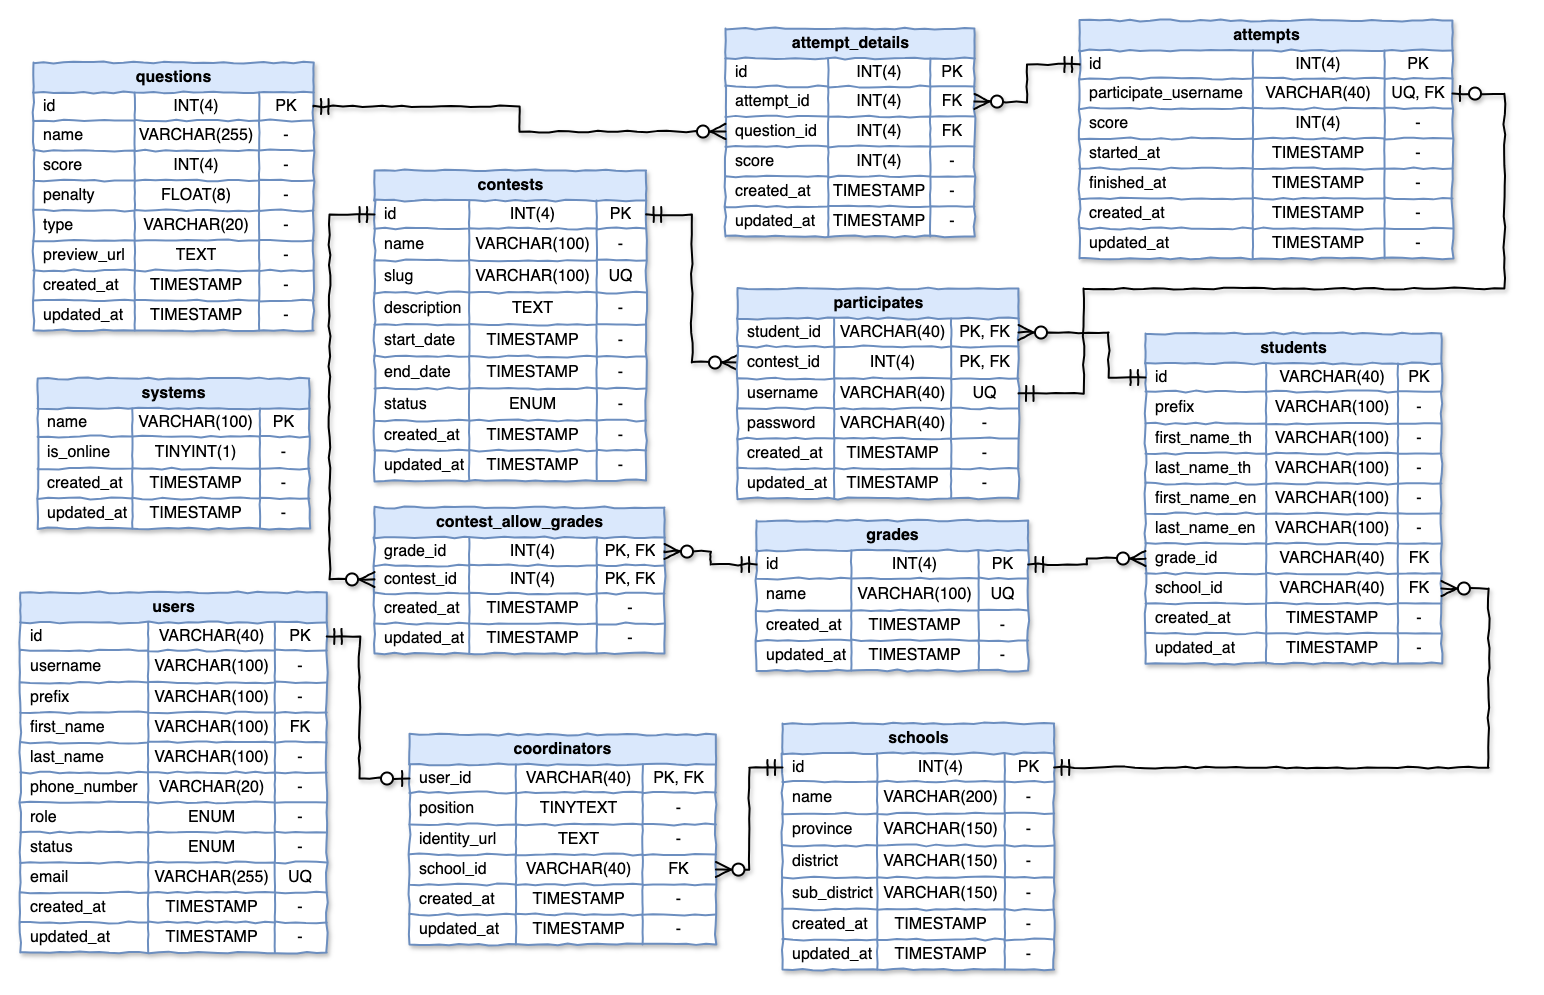
\includegraphics[width=120mm,scale=1.0]{diagrams/database.png}
    \caption{แผนภาพข้อมูลระดับโครงสร้างของฐานข้อมูลในระบบ}
    \label{fig:physical-database-diagram}
\end{figure}

\section{พจนานุกรมข้อมูล (Data Dictionary)}

\subsection{ตารางข้อมูลในระบบ}
\begin{table}[H]
    \caption{ตารางข้อมูลในระบบ พร้อมคำอธิบาย}
    \label{tab:database}
    \begin{tabularx}{\textwidth}{ | p{3cm} | X | }
    \hline
    \textbf{ชื่อตาราง} & \textbf{คำอธิบาย} \\
    \hline
    contests & จัดเก็บประเภทการแข่งขัน \\
    \hline
    grades & จัดเก็บระดับชั้นของนักเรียน \\
    \hline
    schools & จัดเก็บข้อมูลโรงเรียนในประเทศไทย \\
    \hline
    students & จัดเก็บข้อมูลของนักเรียนที่สมัครเข้าแข่งขัน \\
    \hline
    systems & จัดเก็บสถานะการเปิด-ปิดของระบบ \\
    \hline
    users & จัดเก็บข้อมูลส่วนตัวของผู้ใช้ \\
    \hline
    user\_coordinators & จัดเก็บข้อมูลของผู้ใช้ที่เป็นผู้ประสานงานเพื่อยืนยันตัวตน \\
    \hline
    \end{tabularx}
\end{table}
    

\subsection{พจนานุกรมข้อมูลของตาราง}
\begin{table}[H]
    \caption{พจนานุกรมข้อมูลของตาราง contests}
    \label{tab:database-contests}
    \begin{tabularx}{\textwidth}{ | p{2.25cm} | p{2.20cm} | p{2.45cm} | p{2cm} | X | }
    \hline
    \textbf{ชื่อข้อมูล} & \textbf{ประเภทข้อมูล} & \textbf{ขนาดของข้อมูล} & \textbf{ข้อจำกัด} & \textbf{คำอธิบาย} \\
    \hline
    id & int & 4 & primary\_key & รหัสการแข่งขัน \\
    \hline
    name & VARCHAR & 100 & required & ชื่อการแข่งขัน \\
    \hline
    slug & VARCHAR & 100 & required & รอแก้ \\
    \hline
    description & TEXT & 2 - 64Kb & - & คำอธิบายการแข่งขัน \\
    \hline
    start\_date & TIMESTAMP & 4 & required & เวลาที่เริ่มการแข่งขัน \\
    \hline
    end\_date & TIMESTAMP & 4 & required & เวลาที่สิ้นสุดการแข่งขัน \\
    \hline
    status & ENUM & 1 & required  & เวลาที่เริ่มการแข่งขัน \\
    \hline
    created\_at & TIMESTAMP & 4 & - & เวลาที่สร้างข้อมูล \\
    \hline
    updated\_at & TIMESTAMP & 4 & - & เวลาที่แก้ไขข้อมูลล่าสุด \\
    \hline
    \end{tabularx}
\end{table}

\begin{table}[htbp]
    \caption{พจนานุกรมข้อมูลของตาราง grades}
    \label{tab:database-grades}
    \begin{tabularx}{\textwidth}{ | p{2.25cm} | p{2.20cm} | p{2.45cm} | p{2cm} | X | }
    \hline
    \textbf{ชื่อข้อมูล} & \textbf{ประเภทข้อมูล} & \textbf{ขนาดของข้อมูล} & \textbf{ข้อจำกัด} & \textbf{คำอธิบาย} \\
    \hline
    id & VARCHAR & 40 & primary\_key & รหัสระดับชั้น \\
    \hline
    name & VARCHAR & 100 & required & ชื่อระดับชั้น \\
    \hline
    created\_at & TIMESTAMP & 4 & - & เวลาที่สร้างข้อมูล \\
    \hline
    updated\_at & TIMESTAMP & 4 & - & เวลาที่แก้ไขข้อมูลล่าสุด \\
    \hline
    \end{tabularx}
\end{table}

\begin{table}[H]
    \caption{พจนานุกรมข้อมูลของตาราง schools}
    \label{tab:database-schools}
    \begin{tabularx}{\textwidth}{ | p{2.25cm} | p{2.20cm} | p{2.45cm} | p{2.15cm} | X | }
    \hline
    \textbf{ชื่อข้อมูล} & \textbf{ประเภทข้อมูล} & \textbf{ขนาดของข้อมูล} & \textbf{ข้อจำกัด} & \textbf{คำอธิบาย} \\
    \hline
    id & INT & 4 & primary\_key & รหัสโรงเรียน \\
    \hline
    name & VARCHAR & 200 & required & ชื่อโรงเรียน \\
    \hline
    province & VARCHAR & 150 & - & จังหวัด \\
    \hline
    district & VARCHAR & 150 & - & เขต/อำเภอ \\
    \hline
    sub\_district & VARCHAR & 150 & - & แขวง/ตำบล \\
    \hline
    created\_at & TIMESTAMP & 4 & - & เวลาที่สร้างข้อมูล \\
    \hline
    updated\_at & TIMESTAMP & 4 & - & เวลาที่แก้ไขข้อมูลล่าสุด \\
    \hline
    \end{tabularx}
\end{table}

\begin{table}[H]
    \caption{พจนานุกรมข้อมูลของตาราง students}
    \label{tab:database-students}
    \begin{tabularx}{\textwidth}{ | p{2.25cm} | p{2.20cm} | p{2.45cm} | p{2cm} | X | }
    \hline
    \textbf{ชื่อข้อมูล} & \textbf{ประเภทข้อมูล} & \textbf{ขนาดของข้อมูล} & \textbf{ข้อจำกัด} & \textbf{คำอธิบาย} \\
    \hline
    id & VARCHAR & 40 & primary\_key & รหัสนักเรียน \\
    \hline
    prefix & VARCHAR & 100 & required & คำนำหน้า \\
    \hline
    first\_name\_th & VARCHAR & 100 & required & ชื่อจริงภาษาไทย \\
    \hline
    last\_name\_th & VARCHAR & 100 & required & นามสกุลภาษาไทย \\
    \hline
    first\_name\_en & VARCHAR & 100 & required & ชื่อจริงภาษาอังกฤษ \\
    \hline
    last\_name\_en & VARCHAR & 100 & required & นามสกุลภาษาอังกฤษ \\
    \hline
    grade\_id & VARCHAR & 40 & foreign\_key & รหัสระดับชั้น \\
    \hline
    school\_id & VARCHAR & 40 & foreign\_key & รหัสโรงเรียน \\
    \hline
    created\_at & TIMESTAMP & 4 & - & เวลาที่สร้างข้อมูล \\
    \hline
    updated\_at & TIMESTAMP & 4 & - & เวลาที่แก้ไขข้อมูลล่าสุด \\
    \hline
    \end{tabularx}
\end{table}

\begin{table}[H]
    \caption{พจนานุกรมข้อมูลของตาราง systems}
    \label{tab:database-systems}
    \begin{tabularx}{\textwidth}{ | p{2.25cm} | p{2.20cm} | p{2.45cm} | p{2cm} | X | }
    \hline
    \textbf{ชื่อข้อมูล} & \textbf{ประเภทข้อมูล} & \textbf{ขนาดของข้อมูล} & \textbf{ข้อจำกัด} & \textbf{คำอธิบาย} \\
    \hline
    name & VARCHAR & 100 & primary\_key & ชื่อระบบย่อย \\
    \hline
    is\_online & BOOLEAN & 1 & required & สถานะของระบบย่อย \\
    \hline
    created\_at & TIMESTAMP & 4 & - & เวลาที่สร้างข้อมูล \\
    \hline
    updated\_at & TIMESTAMP & 4 & - & เวลาที่แก้ไขข้อมูลล่าสุด \\
    \hline
    \end{tabularx}
\end{table}

\begin{table}[htbp]
    \caption{พจนานุกรมข้อมูลของตาราง users}
    \label{tab:database-users}
    \begin{tabularx}{\textwidth}{ | p{2.25cm} | p{2.20cm} | p{2.45cm} | p{2cm} | X | }
    \hline
    \textbf{ชื่อข้อมูล} & \textbf{ประเภทข้อมูล} & \textbf{ขนาดของข้อมูล} & \textbf{ข้อจำกัด} & \textbf{คำอธิบาย} \\
    \hline
    id & VARCHAR & 40 & primary\_key & รหัสผู้ใช้ \\
    \hline
    username & VARCHAR & 100 & required & ชื่อผู้ใช้ \\
    \hline
    prefix & VARCHAR & 100 & required & คำนำหน้า \\
    \hline
    first\_name & VARCHAR & 100 & required & ชื่อจริงภาษาไทย \\
    \hline
    last\_name & VARCHAR & 100 & required & นามสกุลภาษาไทย \\
    \hline
    phone\_number & VARCHAR & 20 & required & หมายเลขโทรศัพท์ \\
    \hline
    role & ENUM & 1 & - & ระดับของผู้ใช้ \\
    \hline
    status & ENUM & 1 & - & สถานะการยืนยัน \\
    \hline
    created\_at & TIMESTAMP & 4 & - & เวลาที่สร้างข้อมูล \\
    \hline
    updated\_at & TIMESTAMP & 4 & - & เวลาที่แก้ไขข้อมูลล่าสุด \\
    \hline
    \end{tabularx}
\end{table}

\begin{table}[H]
    \caption{พจนานุกรมข้อมูลของตาราง user\_coordinators}
    \label{tab:database-user-coordinators}
    \begin{tabularx}{\textwidth}{ | p{1.75cm} | p{2.20cm} | p{2.45cm} | p{2cm} | X | }
    \hline
    \textbf{ชื่อข้อมูล} & \textbf{ประเภทข้อมูล} & \textbf{ขนาดของข้อมูล} & \textbf{ข้อจำกัด} & \textbf{คำอธิบาย} \\
    \hline
    user\_id & VARCHAR & 40 & primary\_key, foreign\_key & รหัสผู้ใช้ \\
    \hline
    position & TINYTEXT & 1 - 255 & required & ตำแหน่งทางการศึกษา \\
    \hline
    identity\_url & TEXT & 2 - 64Kb & required & ลิงก์ของข้อมูลยืนยันตัวตน \\
    \hline
    school\_id & VARCHAR & 40 & foreign\_key & รหัสโรงเรียน \\
    \hline
    created\_at & TIMESTAMP & 4 & - & เวลาที่สร้างข้อมูล \\
    \hline
    updated\_at & TIMESTAMP & 4 & - & เวลาที่แก้ไขข้อมูลล่าสุด \\
    \hline
    \end{tabularx}
\end{table}

\begin{table}[H]
    \caption{พจนานุกรมข้อมูลของตาราง contest\_allow\_grades}
    \label{tab:database-contest-allow_grades}
    \begin{tabularx}{\textwidth}{ | p{2.15cm} | p{2.20cm} | p{2.45cm} | p{2.15cm} | X | }
    \hline
    \textbf{ชื่อข้อมูล} & \textbf{ประเภทข้อมูล} & \textbf{ขนาดของข้อมูล} & \textbf{ข้อจำกัด} & \textbf{คำอธิบาย} \\
    \hline
    grade\_id & INT & 4 & primary\_key, foreign\_key & รหัสระดับชั้น \\
    \hline
    contest\_id & INT & 4 & primary\_key, foreign\_key & รหัสการแข่งขัน \\
    \hline
    created\_at & TIMESTAMP & 4 & - & เวลาที่สร้างข้อมูล \\
    \hline
    updated\_at & TIMESTAMP & 4 & - & เวลาที่แก้ไขข้อมูลล่าสุด \\
    \hline
    \end{tabularx}
\end{table}
\begin{table}[H]
    \caption{พจนานุกรมข้อมูลของตาราง attempts}
    \label{tab:database-attempts}
    \begin{tabularx}{\textwidth}{ | p{2.25cm} | p{2.20cm} | p{2.45cm} | p{2cm} | X | }
    \hline
    \textbf{ชื่อข้อมูล} & \textbf{ประเภทข้อมูล} & \textbf{ขนาดของข้อมูล} & \textbf{ข้อจำกัด} & \textbf{คำอธิบาย} \\
    \hline
    id & INT & 4 & primary\_key & รหัสของคำตอบในการตอบคำถาม \\
    \hline
    participate\_username & VARCHAR & 40 & foreign\_key & ชื่อผู้ใช้ของผู้เข้าร่วม \\
    \hline
    score & INT & 4 & required & คะแนนรวมของคำตอบ \\
    \hline
    start\_at & TIMESTAMP & 4 & - & เวลาที่เริ่มการแข่งขัน \\
    \hline
    finished\_at & TIMESTAMP & 4 & - & เวลาที่สิ้นสุดการแข่งขัน \\
    \hline
    created\_at & TIMESTAMP & 4 & - & เวลาที่สร้างข้อมูล \\
    \hline
    updated\_at & TIMESTAMP & 4 & - & เวลาที่แก้ไขข้อมูลล่าสุด \\
    \hline
    \end{tabularx}
\end{table}
\begin{table}[H]
    \caption{พจนานุกรมข้อมูลของตาราง attempt-detailsattempt_details}
    \label{tab:database-attempt-details}
    \begin{tabularx}{\textwidth}{ | p{2.25cm} | p{2.20cm} | p{2.45cm} | p{2cm} | X | }
    \hline
    \textbf{ชื่อข้อมูล} & \textbf{ประเภทข้อมูล} & \textbf{ขนาดของข้อมูล} & \textbf{ข้อจำกัด} & \textbf{คำอธิบาย} \\
    \hline
    id & INT & 4 & primary\_key & รหัสรายละเอียดคำตอบในการตอบคำถาม \\
    \hline
    attempt\_id & INT & 4 & foreign\_key & รหัสคำตอบ \\
    \hline
    question\_id & INT & 4 & foreign\_key & รหัสคำถาม \\
    \hline
    score & INT & 4 & required & คะแนนของคำตอบ \\
    \hline
    created\_at & TIMESTAMP & 4 & - & เวลาที่สร้างข้อมูล \\
    \hline
    updated\_at & TIMESTAMP & 4 & - & เวลาที่แก้ไขข้อมูลล่าสุด \\
    \hline
    \end{tabularx}
\end{table}
\begin{table}[H]
    \caption{พจนานุกรมข้อมูลของตาราง participates}
    \label{tab:database-participates}
    \begin{tabularx}{\textwidth}{ | p{2.25cm} | p{2.20cm} | p{2.45cm} | p{2.15cm} | X | }
    \hline
    \textbf{ชื่อข้อมูล} & \textbf{ประเภทข้อมูล} & \textbf{ขนาดของข้อมูล} & \textbf{ข้อจำกัด} & \textbf{คำอธิบาย} \\
    \hline
    student\_id & VARCHAR & 40 & primary\_key, foreign\_key & รหัสนักเรียน \\
    \hline
    contest\_id & INT & 4 & primary\_key, foreign\_key & รหัสการแข่งขัน \\
    \hline
    username & VARCHAR & 40 & required & ชื่อผู้ใช้ \\
    \hline
    password & VARCHAR & 40 & required & รหัสผ่าน \\
    \hline
    created\_at & TIMESTAMP & 4 & - & เวลาที่สร้างข้อมูล \\
    \hline
    updated\_at & TIMESTAMP & 4 & - & เวลาที่แก้ไขข้อมูลล่าสุด \\
    \hline
    \end{tabularx}
\end{table}

\begin{table}[H]
    \caption{พจนานุกรมข้อมูลของตาราง questions}
    \label{tab:database-questions}
    \begin{tabularx}{\textwidth}{ | p{2.25cm} | p{2.20cm} | p{2.45cm} | p{2cm} | X | }
    \hline
    \textbf{ชื่อข้อมูล} & \textbf{ประเภทข้อมูล} & \textbf{ขนาดของข้อมูล} & \textbf{ข้อจำกัด} & \textbf{คำอธิบาย} \\
    \hline
    id & INT & 4 & primary\_key & รหัสคำถาม \\
    \hline
    name & VARCHAR & 255 & required & ชื่อคำถาม \\
    \hline
    score & INT & 4 & required & คะแนนคำถาม \\
    \hline
    penalty & FLOAT & 8 & required & คะแนนที่ลบ \\
    \hline
    type & VARCHAR & 20 & required & ประเภทคำถาม \\
    \hline
    preview\_url & 20 & required & ลิงก์เพื่ออ่านคำถาม \\
    \hline
    created\_at & TIMESTAMP & 4 & - & เวลาที่สร้างข้อมูล \\
    \hline
    updated\_at & TIMESTAMP & 4 & - & เวลาที่แก้ไขข้อมูลล่าสุด \\
    \hline
    \end{tabularx}
\end{table}

